\section{Datenmodell}
\setauthor{Hain Lukas}

\begin{figure}[H]
    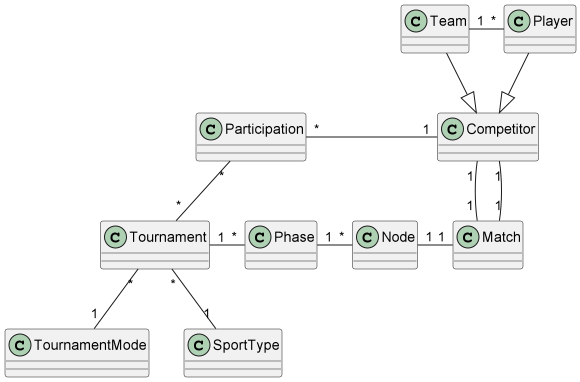
\includegraphics[scale=1]{pics/class_diagram.png}
    \caption{Class Diagram}
\end{figure}

Oben abgebildet ist das Datenmodell der Quarkus Applikation. Anfangs erstellt man ein Turnier (Tournament), neben Namen, Startdatum und Enddatum 
wird hier noch der Turniermodus (TournamentMode) und die Sportart (SportType) festgelegt. Nun gibt man an, welche Teilnehmer (Competitor) an diesem Turnier teilnehmen (Participation). 
Ein Competitor kann entweder ein einzelner Spieler (Player) oder ein Team von Spielern (Team) sein.
Wenn das Turnier gestartet wird, wird das Turnier in Phasen (Phase) unterteilt. In jeder Phase gibt es eine bestimmte Anzahl an Matches (Match), welche jeweils 2 Competitor haben und mithilfe von Nodes (Node) 
der jeweiligen Phase zugeordnet werden.

\section{Quarkus Applikation}
\setauthor{Hain Lukas}

\begin{figure}[H]
    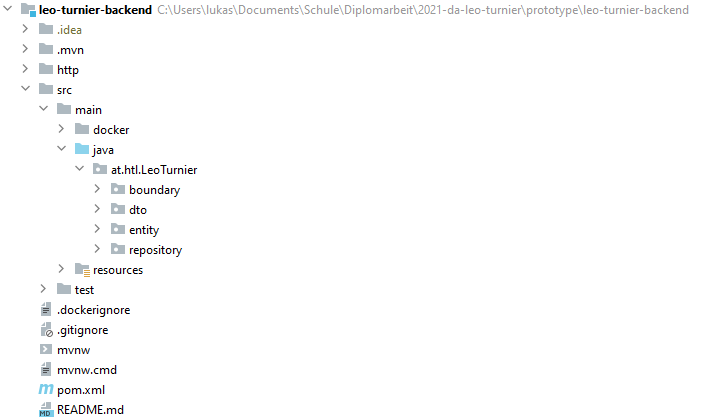
\includegraphics[scale=0.8]{pics/quarkus_file_structure.png}
    \caption{Quarkus Ordnerstruktur}
\end{figure}

(Ist dieser Teil zu Basic?)

Nach dem erstellen einer Quarkus Applikation ist ein Großteil der Ordnerstruktur bereits im vorhinein gegeben. Das wichtigste File im Projekt befindet sich ganz im äußersten Ordner, nämlich das "pom.xml" File. Hier werden 
nicht nur die Metadaten des Projekts angegeben, sondern auch die Dependencies, also alle externen Libraries, die die Applikation benötigt. 
Im "src" Ordner befinden sich ein "main" und ein "test" Ordner. Im "main" Ordner befindet sich der ganze Quellcode der Applikation, und im "test" Ordner befindet sich der Code, der den Quellcode auf seine richtigkeit prüft.
Im "main" Ordner befindet sich nun ein "docker" Ordner, auf den später noch eingegangen wird, ein "java" Ordner, in dem sich die Java Klassen der Applikation befindet, und ein "resources" Ordner, in dem weitere Files zu finden sind, 
auf die der Java Code eventuell zugreifen kann.

Die Java Klassen im "java" Ordner sind weiters in 4 verschiedene Ordner aufgeteilt. Im "entity" Ordner befinden sich alle Entitätsklassen der Applikation, also jene, die das Datenmodell (siehe Kapitel 6.1 Datenmodell) wiederspiegeln.
Die Klassen im "repository" sind die Schnittstelle zwischen der Quarkus Applikation und der Datenbank. Sie sind für die CRUD Operationen verantwortlich, also das Speichern, Auslesen, Verändern oder Löschen von Daten nach dem Schema der Entitätsklassen.
Außerdem befindet sich hier die Logik hinter den Turnieren. Die Klassen im "boundary" sind die Schnittstelle zum Frontend. Sie nehmen Requests, also Anforderungen, von außen an, 
führen die jeweilige Methode aus den Repository Klassen aus und liefern dann eine Response, also eine Antwort, zurück. Zuletzt gibt es noch die Klassen in "dto" Ordner, diese sind Klassen, in denen Daten gespeichert werden können, die für die Logik in den 
Repository Klassen benötigt wird, jedoch nicht unbedingt Teil des Datenmodells sind.
 